\tikzstyle{processstep}=[draw,text width=3.5cm,text centered,minimum width=4cm,minimum height=1cm]
\tikzstyle{orientedarc}=[->,>=latex]

\tikzstyle{justleft}=[shift={(-0.5cm,0cm)}]
\tikzstyle{justright}=[shift={(0.5cm,0cm)}]
\tikzstyle{justtop}=[shift={(0cm,0.5cm)}]
\tikzstyle{justdown}=[shift={(0cm,-0.5cm)}]



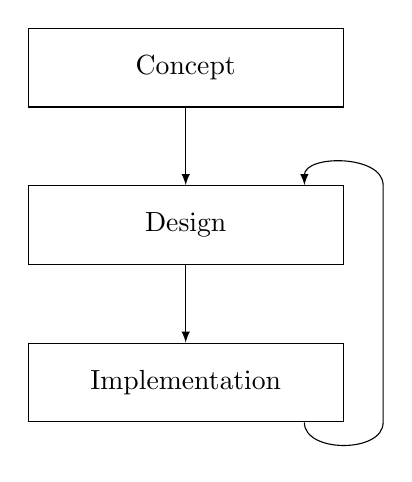
\begin{tikzpicture}

\node[processstep] (S1) at (0cm,4cm) {Concept};
\node[processstep] (S2) at (0cm,2cm) {Design};
\node[processstep] (S3) at (0cm,0cm) {Implementation};

\coordinate[justright] (S2NORTHEAST1) at (S2.north east);
\coordinate[justright] (S2SOUTHEAST1) at (S2.south east);
\coordinate[justleft] (S2NORTHEAST2) at (S2.north east);
\coordinate[justleft] (S2SOUTHEAST2) at (S2.south east);

\coordinate[justright] (S3NORTHEAST1) at (S3.north east);
\coordinate[justright] (S3SOUTHEAST1) at (S3.south east);
\coordinate[justleft] (S3NORTHEAST2) at (S3.north east);
\coordinate[justleft] (S3SOUTHEAST2) at (S3.south east);

\draw[orientedarc] (S1) -- (S2);
\draw[orientedarc] (S2) -- (S3);
\draw[orientedarc] (S3SOUTHEAST2) to[bend right=90] (S3SOUTHEAST1) -- (S2NORTHEAST1) to[bend right=90] (S2NORTHEAST2);

\end{tikzpicture}
